\problemname{Pickle Clicker}
\noindent

Approximately six months ago, the critically acclaimed game \emph{Pickle Clicker} was released.
After spending countless hours on the game, Rasmus has decided to take things to the
next level: he plans to speedrun the game.

The goal of Pickle Clicker is to collect as much of the currency pickles as possible. The
goal in a speedrun is to purchase the Megapickle as quickly as possible, which costs
$T$ pickles. In the game, there are also $N$ different types of buildings. The various
types are numbered from $1$ to $N$, where the $i$-th type produces $p_i$ pickles per
second and costs $c_i$ pickles to build.

\textit{At the start, you own a building of type $1$}. Every second, the following events occur:

\begin{enumerate}
  \item Every building you own produces pickles. A building of type $i$ produces $p_i$ pickles.
  \item Afterwards, you have the option to buy a building or buy the Megapickle. A building
  of type $i$ costs $c_i$ pickles to build, and you must afford it to be able to buy it.
  You can buy a maximum of one building per second, and it is allowed to have multiple
  buildings of the same type.
\end{enumerate}

Help Rasmus determine how to play the game so that he can purchase the Megapickle in as
few seconds as possible. See the example below to get a clearer understanding of the rules.

\section*{Input}
The first line of input contains the integers $N$ and $T$ ($1 \le N \le 6$, $1 \leq T \leq 10^5$),
the number of buildings and the cost of the Megapickle.

The following $N$ lines each contain the integers $p_i, c_i$ ($1 \leq p_i, c_i \leq T$),
describing the production speed and cost of the $i$-th building type.

\section*{Output}
Print an integer: the number of seconds it takes to win Pickle Clicker if you play optimally.

\section*{Points}
Your solution will be tested on several test case groups.
To get the points for a group, it must pass all the test cases in the group.

\noindent
\begin{tabular}{| l | l | p{12cm} |}
  \hline
  \textbf{Group} & \textbf{Point value} & \textbf{Constraints} \\ \hline
  $1$    & $20$       & $N=1$ \\ \hline
  $2$    & $20$       & $T \leq 10$ \\ \hline
  $3$    & $20$       & $T \leq 1000$ \\ \hline
  $4$    & $40$       & No additional constraints. \\ \hline
\end{tabular}

\section*{Sample explanation}

\begin{figure}[h]
  \centering
  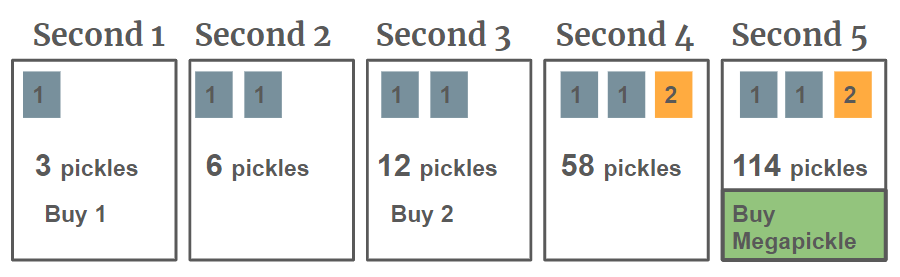
\includegraphics[width=0.7\textwidth]{sample1-en.PNG}
    \\The image shows the solution to sample 1. The first row describes which buildings 
    we own at the start of the corresponding second. The second row is how many pickles 
    we have after the buildings have produced. The last row indicates whether we bought
    something at the end of the second.
  
\end{figure}
